\begin{savequote}[75mm] 
Let’s keep the night fantastic\\
Light it up, tell me more, explore
\qauthor{``Who Do We Think We Are?''- John Legend} 
\end{savequote}

\chapter{Exploratory Analysis}
Before performing any modeling, we first examined the feasibility of two potential approaches to our problem in terms of the type of data used, a \textit{network-based} approach, using cover song data v. a \textit{content-based} approach, using song audio directly.

\section{Analysis of Network Data}
\subsection{AllMusic Influence Network}
The AllMusic influence network is a sparse graph consisting of 16,704 artists and 93,065 influence relationships with each artist having an average of 5.57 followers. Both the indegree and degree distributions are heavily right skewed, which makes intuitive sense as most artists have relatively few followers, while extremely influential artists have many followers.

\begin{figure}
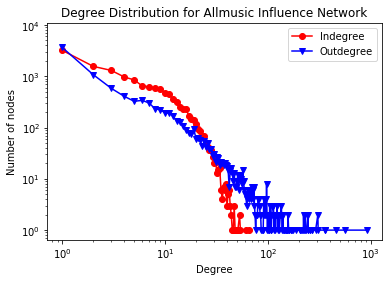
\includegraphics[width=\textwidth]{figures/allmusic_degree_distribution.png}
\caption{Degree distributions for AllMusic influence network}
\end{figure}

\subsubsection*{Highest Out-Degree Artists}
Ordered by degree, the top 25 artists that directly influenced the highest number of followers are listed in Table 1, followed by the count of artists they influenced.


\begin{table}[H]
\centering
\caption{Artists with highest degree in AllMusic influence network}
\label{my-label}
\begin{tabular}{lr}
\hline
 Artist                 &   out-degree \\
\hline
 The Beatles            &         911 \\
 Bob Dylan              &         558 \\
 The Rolling Stones     &         463 \\
 David Bowie            &         358 \\
 The Velvet Underground &         356 \\
 Jimi Hendrix           &         308 \\
 The Beach Boys         &         306 \\
 The Kinks              &         306 \\
 Led Zeppelin           &         291 \\
 Neil Young             &         269 \\
 Miles Davis            &         266 \\
 James Brown            &         260 \\
 The Byrds              &         259 \\
 Black Sabbath          &         245 \\
 John Coltrane          &         244 \\
 Hank Williams          &         243 \\
 The Stooges            &         241 \\
 Brian Eno              &         237 \\
 The Who                &         230 \\
 Pink Floyd             &         227 \\
 Ramones                &         225 \\
 The Clash              &         224 \\
 Kraftwerk              &         222 \\
 Elvis Presley          &         222 \\
 Sex Pistols            &         220 \\
\hline
\end{tabular}
\end{table}

The genre of rock has the highest representation in this list, with artists from jazz, electronic and pop appearing as well.


\subsubsection*{Breakdown by Genre}
\begin{table}[H]
\centering
\caption{Proportion of artists belonging to each genre}
\label{my-label}
\begin{tabular}{lr}
\hline
Genre &  Proportion \\
\hline
Pop/Rock       &    0.430136 \\
Jazz           &    0.087524 \\
R\&B;           &    0.065852 \\
Unknown        &    0.065254 \\
Rap            &    0.057890 \\
Electronic     &    0.057771 \\
Country        &    0.044959 \\
Latin          &    0.025682 \\
Blues          &    0.024545 \\
International  &    0.020175 \\
Vocal          &    0.018738 \\
Folk           &    0.018259 \\
Religious      &    0.016403 \\
Reggae         &    0.015805 \\
Classical      &    0.015386 \\
Comedy/Spoken  &    0.010836 \\
Avant-Garde    &    0.007663 \\
New Age        &    0.006765 \\
Stage \& Screen &    0.006645 \\
Easy Listening &    0.002814 \\
Children's     &    0.000838 \\
Holiday        &    0.000060 \\
\hline
\end{tabular}
\end{table}

Unsurprisingly, we see that Pop/Rock is over represented in this data set, followed by Jazz R\&B, Rap, Electronic and Country. 6.5\% of artists do not have genre labels associated with them.

\subsubsection{Influence Between Genres}
To visualize the amount of influence between genres as represented by the AllMusic influence graph, we created the heatmap in the figure below:

\begin{figure}[H]
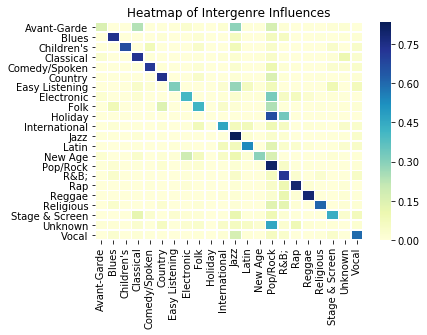
\includegraphics[width=\textwidth]{figures/heatmap.png}
\caption{Heatmap of intergenre influence in AllMusic influence graph}
\end{figure}

In order to construct the heatmap, we used the genre metadata we scraped for each artist, using the first genre tag for artists with multiple genre tags to calculate the frequencies of edges from each genre to every other genre, normalizing by the total number of edges originating from each genre. Therefore the heatmap can be read as follows: row $M$ column $N$ designates the proportion of influence genre $M$ contributes to genre $N$ (darker hue meaning higher contribution) as suggested by the network graph, with the proportions in each row summing to $1$ and the diagonal entries indicating how self-contained or ``insular'' a genre is.

We observe that:
\begin{itemize}
    \item A majority of genres give their second highest influence contribution (outside of to themselves) to Pop/Rock, which is not surprising given the conglomerate nature of Pop/Rock as a genre
    \item Avant-Garde is relatively evenly spread in its influence between itself, Classical, Jazz and Pop/Rock
    \item Jazz, Pop/Rock and Rap appear to be the most ``insular'' genres
    \item Blues influences Jazz, Pop/Rock and R\&B, which is consistent with conventional wisdom
\end{itemize}

It is important to note the limitations of using genre information from AllMusic. First, we note that Pop/Rock are lumped into one category, which is not ideal as two discrete categories for the two genres would be more informative. Secondly, since AllMusic reflects popular music tastes across the past century, we see over-representation of artists from genres such as Jazz and Pop/Rock in the influence graph, which skews results in the heatmap as well.

\subsection{SecondHandSongs Covers}
After dropping covers with missing performer and release date information from the SHS cover data, we were left with 644,786 total versions (covers) of 86,827 unique works from 77,328 unique artists.

\subsubsection*{Distribution of Number of Covers per Work}
Grouping versions together by the original work they are associated with, we calculated basic summary statistics:

\begin{table}[H]
\centering
\caption{Summary statistics for number of covers per original work from SecondHandSongs}
\label{my-label}
\begin{tabular}{lr}
count &  86827.00000 \\
mean  &      7.42610 \\
std   &     25.23396 \\
min   &      1.00000 \\
25\%   &      2.00000 \\
50\%   &      2.00000 \\
75\%   &      5.00000 \\
max   &   2004.00000 \\
\end{tabular}
\end{table}

This distribution is also heavily right-skewed, with a median count of 2 covers per original work and a mean of 7.426.

\subsubsection*{Most Covered Works}
We extracted the top 25 most covered works from SecondHandSongs, along with counts of the number of times they were covered.

\begin{table}[H]
\centering
\caption{Most covered works from SecondHandSongs}
\label{my-label}
\begin{tabular}{lr}
\hline
 Work Name                                         &   Covers \\
\hline
 Silent Night! Holy Night!                         &     2004 \\
 Summertime                                        &     1611 \\
 Away in a Manger [Mueller]                        &     1536 \\
 O, Holy Night                                     &     1304 \\
 New Britain                                       &      858 \\
 White Christmas                                   &      828 \\
 Have Yourself a Merry Little Christmas            &      825 \\
 O Come, All Ye Faithful                           &      808 \\
 Can't Help Falling in Love                        &      804 \\
 The Christmas Song (Merry Christmas to You)       &      761 \\
 Over the Rainbow                                  &      709 \\
 Body and Soul                                     &      707 \\
 What Child Is This?                               &      664 \\
 Winter Wonderland                                 &      615 \\
 God Rest You Merry, Gentlemen                     &      612 \\
 Jingle Bells                                      &      608 \\
 The First Nowell the Angel Did Say                &      605 \\
 My Funny Valentine                                &      579 \\
 Stille Nacht! Heilige Nacht!                      &      545 \\
 Yesterday                                         &      538 \\
 I'll Be Home for Christmas (If Only in My Dreams) &      538 \\
 Carol of the Drum                                 &      534 \\
 Joy to the World                                  &      531 \\
 St. Louis Blues                                   &      521 \\
 Love Me Tender                                    &      520 \\
\hline
\end{tabular}
\end{table}

We see highest representation from Christmas songs and jazz standards in this list. 


\subsection{MusicBrainz Collaboration Network}
The MusicBrainz collaboration network is an undirected graph consisting of 271,442 nodes (artists) and 650,920 edges with average degree 4.796. The graph is not connected and instead consists of 26,654 separate connected components.

\subsection{Overlap Analysis Between Datasets}
\subsubsection{Overlap Between Influence Network and Cover Songs}
We first calculated the node overlap between the AllMusic influence network and artist names in the SecondHandSongs dataset using exact string matching. The node overlap found using this method was 57.24\%, which perhaps reflects the limitations of this approach.

We also calculated edge overlap between the influence network and the cover songs data. Obviously, the cover song data does not form a network on its own. In fact, one natural way of viewing the sequence of covers for a given original work is that each cover sequence is an observed \textit{trace} of information diffusion across a latent directed network of influence between musicians. 

Therefore we used three different underlying assumptions for network formation in order to establish a baseline for edge overlap between the influence and cover song data:
\begin{enumerate}
    \item \textit{Next immediate chronological neighbor}: creating directed edges between each artist and the next immediate artist chronologically that covered the same original work
    \item \textit{First artist to each successor}: creating directed edges between the first artist that covered an original work and each of the subsequent artists who covered the original work
    \item \textit{Each artist to every possible successor}: creating directed edges between each artist and every subsequent artist in the cover sequence for the song
\end{enumerate}

The edge overlaps between AllMusic and SHS for each of these edge creation assumptions are summarized in the table below:

\begin{table}[H]
\centering
\caption{Edge overlap based on cover song edge creation assumption}
\label{my-label}
\begin{tabular}{|l|l|l|}
\hline
Assumption & Number of Edges Overlap & Percentage Overlap \\ \hline
1      & 2951                    & 3.55\%             \\ \hline
2      & 6461                    & 7.77\%             \\ \hline
3      & 14668                   & 17.6\%             \\ \hline
\end{tabular}
\end{table}


Assumption (3) yielded the highest overlap, which is not surprising given that it generates the highest number of possible ``edges''. Allowing for duplicates (2 artists who were in the same cover sequence for multiple songs), assumption (3) yielded 82,558 ``edges'' that were found in the ground truth, which means that artists will often cover their influencers' original works more than just once.

Overall, the percentage overlap is not very high for any of the methods. One possible reason is the imperfect approach of using exact string matching on artist names between the two datasets, so there may be discrepancies created by handling of special characters, alternate spellings, variations of artist names etc.

\subsubsection{Overlap Between Influence Network and Collaboration Network}
We also calculated the node and edge overlap between the AllMusic influence network and the MusicBrainz collaboration network. Again, we used exact string matching on artist name between the two datasets.

The node (artist name) overlap between the two datasets is 63.69\%, which is comparable to the artist name overlap between AllMusic and SHS. By overlap, we refer to the number of artist names in the smaller influence network that are found in the collaboration network divided by the total number of nodes in the influence network.

We also calculated edge overlap between the two datasets. Since the collaboration network is undirected, for each undirected edge $(u,v)$ in the graph, we introduced two directed edges $(u,v)$ and $(v,u)$ for the purpose of calculating overlap. The calculated overlap is 3.53\%, which is far lower than the overlap between the influence network and cover songs data. This simple heuristic suggests that collaboration relationships are not especially directly predictive of influence relationships, which is reasonable given that many musicians never get the opportunity to record with their influences.

\subsection{Limitations of Network-based Approach}
Regardless of the method used to construct a network out of cover song data, whether one of the heuristics mentioned in 3.4 or a cascade-based influence algorithm such as in \cite{gomez2010inferring}, the use of cover song data arguably poses two fundamental challenges in influence inference, which we will refer to as the \textbf{standards effect} and the \textbf{career cover artist effect}.

By the standards effect, we mean that certain songs are covered very often simply because they are a common part of the repertoire (think Christmas songs or jazz standards). This behavior obscures true influence relationships and is commonly referred to in network terminology as \textbf{herding}. Evidence for this phenomenon can be seen in Table 4, where we see that many of the most covered works are precisely Christmas songs or jazz standards. By the career cover artist effect, we refer to the fact that certain artists almost exclusively record cover songs, where the covers are often recorded for commercial reasons or other non-influence reasons.

These issues could be dealt with through certain heuristics, for example removing songs that have over a certain number of covers. However, combined with the poor node overlap issue, perhaps this suggests that a network-based approach using cover songs is not the best way to address our task due to the underlying signal being too weak.

\section{Analysis of Audio Data}
\subsection{Coverage}
Since we scraped the audio data directly from the AllMusic website matching on the unique Artist identifier for the site, we did not run into the coverage overlap issues that we did with the cover song or collaboration datasets. We were able to collect audio clips for 92.55\% of artists in the AllMusic influence network, which accounts for 95.64\% of the influence edges in the ground truth influence dataset. 

We were able to extract a mean of 9.29 30-second long clips per artist, with less than 14\% of artists having less than 10 audio clips and less than 7\% having less than 5 clips. In total, 143,625 clips of audio were collected.

\subsection{Intermediate Feature Representation}
The raw audio files are far too large to use directly and high-level engineered features such as those used in \cite{shalit2013modeling} can be overly lossy. Therefore we struck a balance between these extremes through the use of 2 types of intermediate time-frequency feature representations commonly \cite{van2013deep} used in audio signal processing, \textbf{Mel-Spectrograms} and \textbf{Mel-frequency Cepstral Coefficients} (\textbf{MFCCs}). The \textbf{mel scale} performs a logarithmic transformation of frequencies to more closely approximate the way humans perceive pitch distances.

\begin{figure}[H]
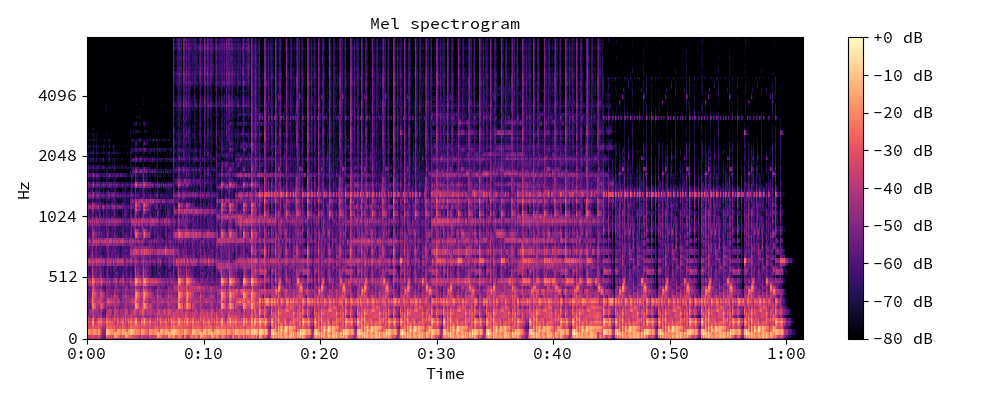
\includegraphics[width=\textwidth]{figures/melspec.png}
\caption{Example of Mel-Spectrogram representation of audio file}
\end{figure}

\begin{figure}[H]
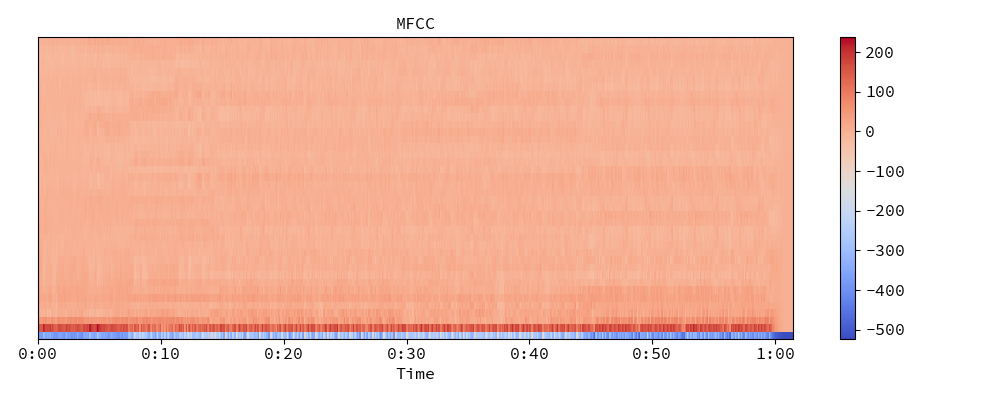
\includegraphics[width=\textwidth]{figures/mfcc.png}
\caption{Example of MFCC representation of audio file}
\end{figure}


\subsection{Dimensionality Reduction with PCA}
We used Principal Component Analysis (PCA) for dimensionality reduction. PCA takes a set of data and transforms it into a new orthonormal coordinate system where the first coordinate (first principal component) explains the most variance, the second principal component explains the second most variance and so on.

Taking the MFCC features corresponding to the first AllMusic audio sample for each artist, we extracted the first 2 principal components, which together explained approximately 55 percent of the variance in the data. We then visualized the projection of the MFCC features onto the first two principal components, colored by genre and with text labels for the top 3 highest out-degree artists per genre. For increased readability, we only included data points from the 7 most popular genres in terms of total number of artists. The visualization can be seen in Figure 4.

\newpage
\begin{figure}[H]
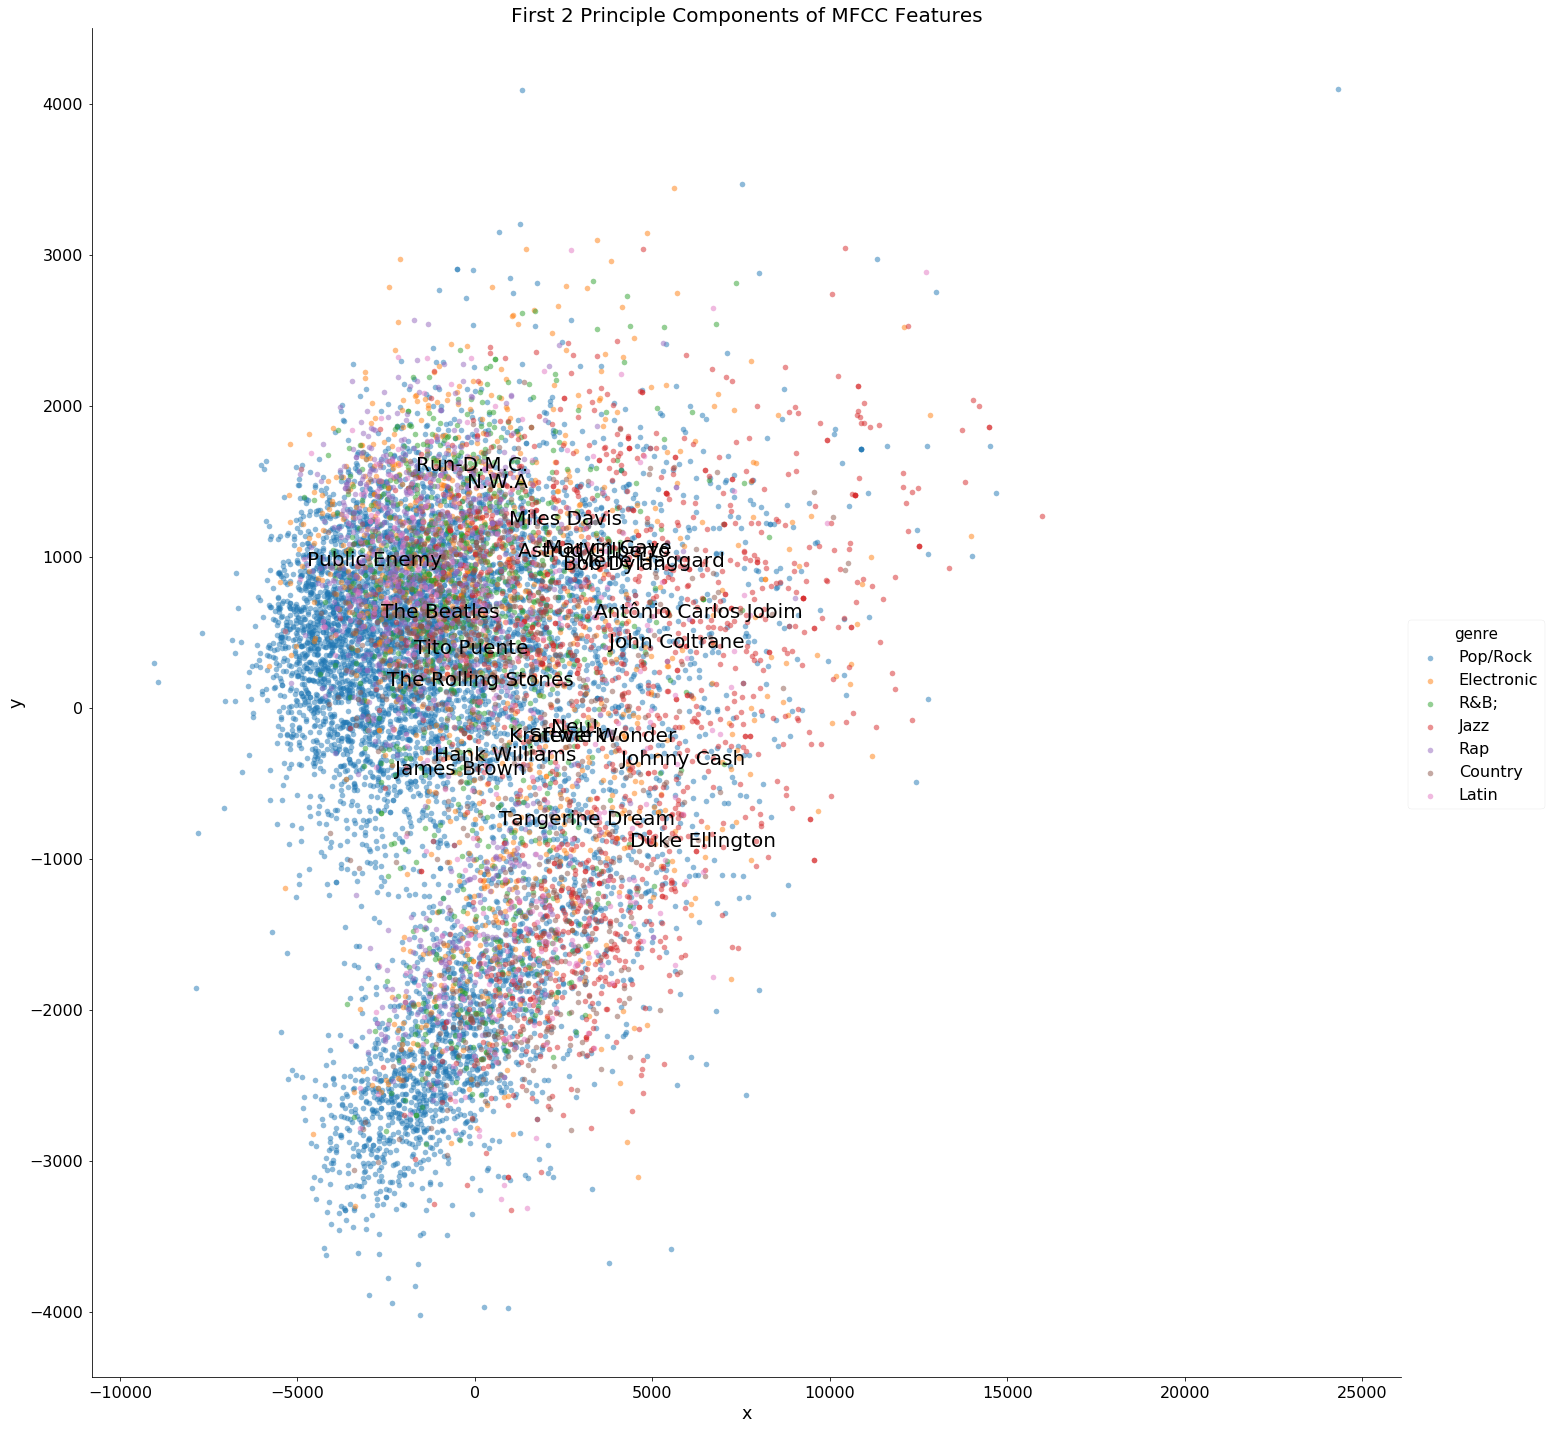
\includegraphics[width=15cm]{figures/mfcc_pca.png}
\caption{PCA projection of MFCC features}
\end{figure}

\newpage

Note that we only used one 30 second clip to represent each artist, but even so there are readily discernible patterns. The highest degree Rap artists, N.W.A., Run-D.M.C. and Public Enemy are all localized to the top left of the plot, where there appears to be a large cluster of other Rap artists. The Jazz genre seems to be predominantly located in the right half of the plot while the bulk of R\&B is located between Rap and Jazz, which is consistent with both the chronology and stylistic progression relationship between these three genres.

\subsection{Relationship Between Influence Graph Distance \& Euclidean Distance on PC Projection}
We also investigated the relationship between node distance in the AllMusic Influence Graph and Euclidean distance in the principal component projection. To do this we computed the average Euclidean distance in the principal component projection between each artist and all descendants at BFS distance exactly $d$ followers away in the influence graph for increasing values of $d$. 

\begin{figure}[H]
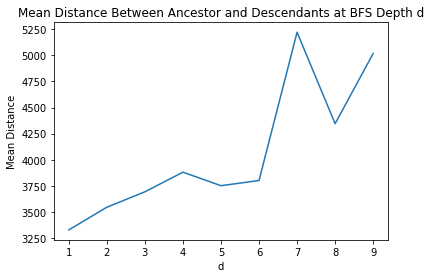
\includegraphics[width=10cm]{figures/distance_by_bfs.png}
\caption{Average Euclidean distance between nodes in PC plot v. BFS depth in influence graph}
\end{figure}

We see that mean Euclidean distance roughly increases with increasing BFS depth, which provides evidence that the PCA projection structure approximately corresponds to the influence network in terms of influencer-follower distance. 

Overall, from our exploratory analysis we saw that there were many limitations to using a network-based approach and that the content-based approach appeared more promising. Therefore, we decided to focus on content-based approaches, which will be the focus of the remainder of this thesis.